%------------------- BOLT ANALYSIS -------------------%
\subsection{Fasteners} \label{subsec:bolt_analysis}


%------------------------------ Inputs and Outputs ------------------------------%
\subsubsection{Inputs and Outputs}

Inputs include the number of bolts $n$, distance $P$ from the applied forces to the centroid, distance from the bolt to centroid $r$, and angles $\rho$ and $\epsilon$ between $P$ and $x$ around $z$ and $y$ respectively.
The minimum acceptable bolt diameter $d$ and distance from bolt to member edge $\ell$ are then calculated.


%------------------------------ CONSTANTS and Parameters ------------------------------%
\subsubsection{Constants and Parameters}

A safety factor of 2.5 was selected.
This is in accordance with the recommendations provided by Juvinall and Marshek for average materials operating in ordinary environmental conditions, subjected to loads and stresses that can be determined \cite{juvinall_fundamentals_2012}.
Since the maximum stresses have been simulated, the maximum stresses can be determined with relative accuracy, however due to the uncertainty of vandalism, a smaller safety factor was not selected; thus 2.5 strikes a solid balance between being conservative and still flexible.
A safety factor for tension is specific has been set at 2; as shown in the example below, the initial bolt tension sets the safety factor at $2.3$, so the actual value will be $2.3$ or smaller depending on the applied load.
Bolt properties are also constant and are found in Table \ref{tab:bolts_material}


%------------------------------ ASSUMPTIONS/SIMPLIFICATIONS ------------------------------%
\subsubsection{Assumptions and Simplifications}

The following assumptions were made while analysing the bolts at the hips:

\begin{enumerate}
    \item Absolutely rigid members \cite{budynas_shigleys_2015}
    \item Ductile bolt material
    \item Negligible impact loading and vibrations
    \item Washers do not greatly influence the found safety factor, and are therefore not included in the analysis
    \item Bolt threaded and unthreaded length can be customized and do not need to follow the formulation provided in Shigley or Juvinall
    \item Fatigue loading is negligible
    \item Load due to tensile moment is evenly distributed between all bolts (which would in reality become larger the further form the pivot point the bolt is)
\end{enumerate}

%------------------------------ MATERIAL SELECTION ------------------------------%
\subsubsection{Material Selection}

SAE class 9.8 medium carbon bolts were pre-emptively selected as they cover a large swath of diameters (M1.6-M16), have good tensile and proof strength, and are not as expensive as higher class bolts.
Environmental resistance is not paramount as all bolts are contained within the chassis or bellows, however since condensation is likely, some degree of protection against corrosion is necessary.
Coarse-tooth bolts were selected. Although fine tooth bolts have higher tensile area, allowing for smaller diameter bolts, and are less likely to loosen over time, their availability in sizes below M8 seem severely limited \cite{budynas_shigleys_2015} \cite{nord-lock_group_should_2010}.

\begin{table}[H]
    \centering
    \caption{Properties of ISO Class 9.8 Bolts}
    \label{tab:bolts_material}
    \begin{tabular}{l c}
        \\ \hline
        \textbf{Property} & \textbf{Measure}
        \\ \hline
        Bolt sizes & M1.6-M16
        \\
        Proof Strength $S_p$ & $650\text{ MPa}$
        \\
        Yield Strength $S_y$ & $720\text{ MPa}$
        \\
        Tensile Strength $S_{ut}$ & $900\text{ MPa}$
        \\
        Endurance Strength $S_e$ & $140\text{ MPa}$
        \\
        Fatigue Stress-Concentration Factor $k_f$ & $3.8$ (Cut Threads)
        \\ \hline
    \end{tabular}
\end{table}


%------------------------------ FREE BODY DIAGRAM ------------------------------%
\subsubsection{Free-Body Diagram}

The general Free-Body Diagram is shown in Figure \ref{fig:bolt_fbd_general}.

\begin{figure}
    \centering
    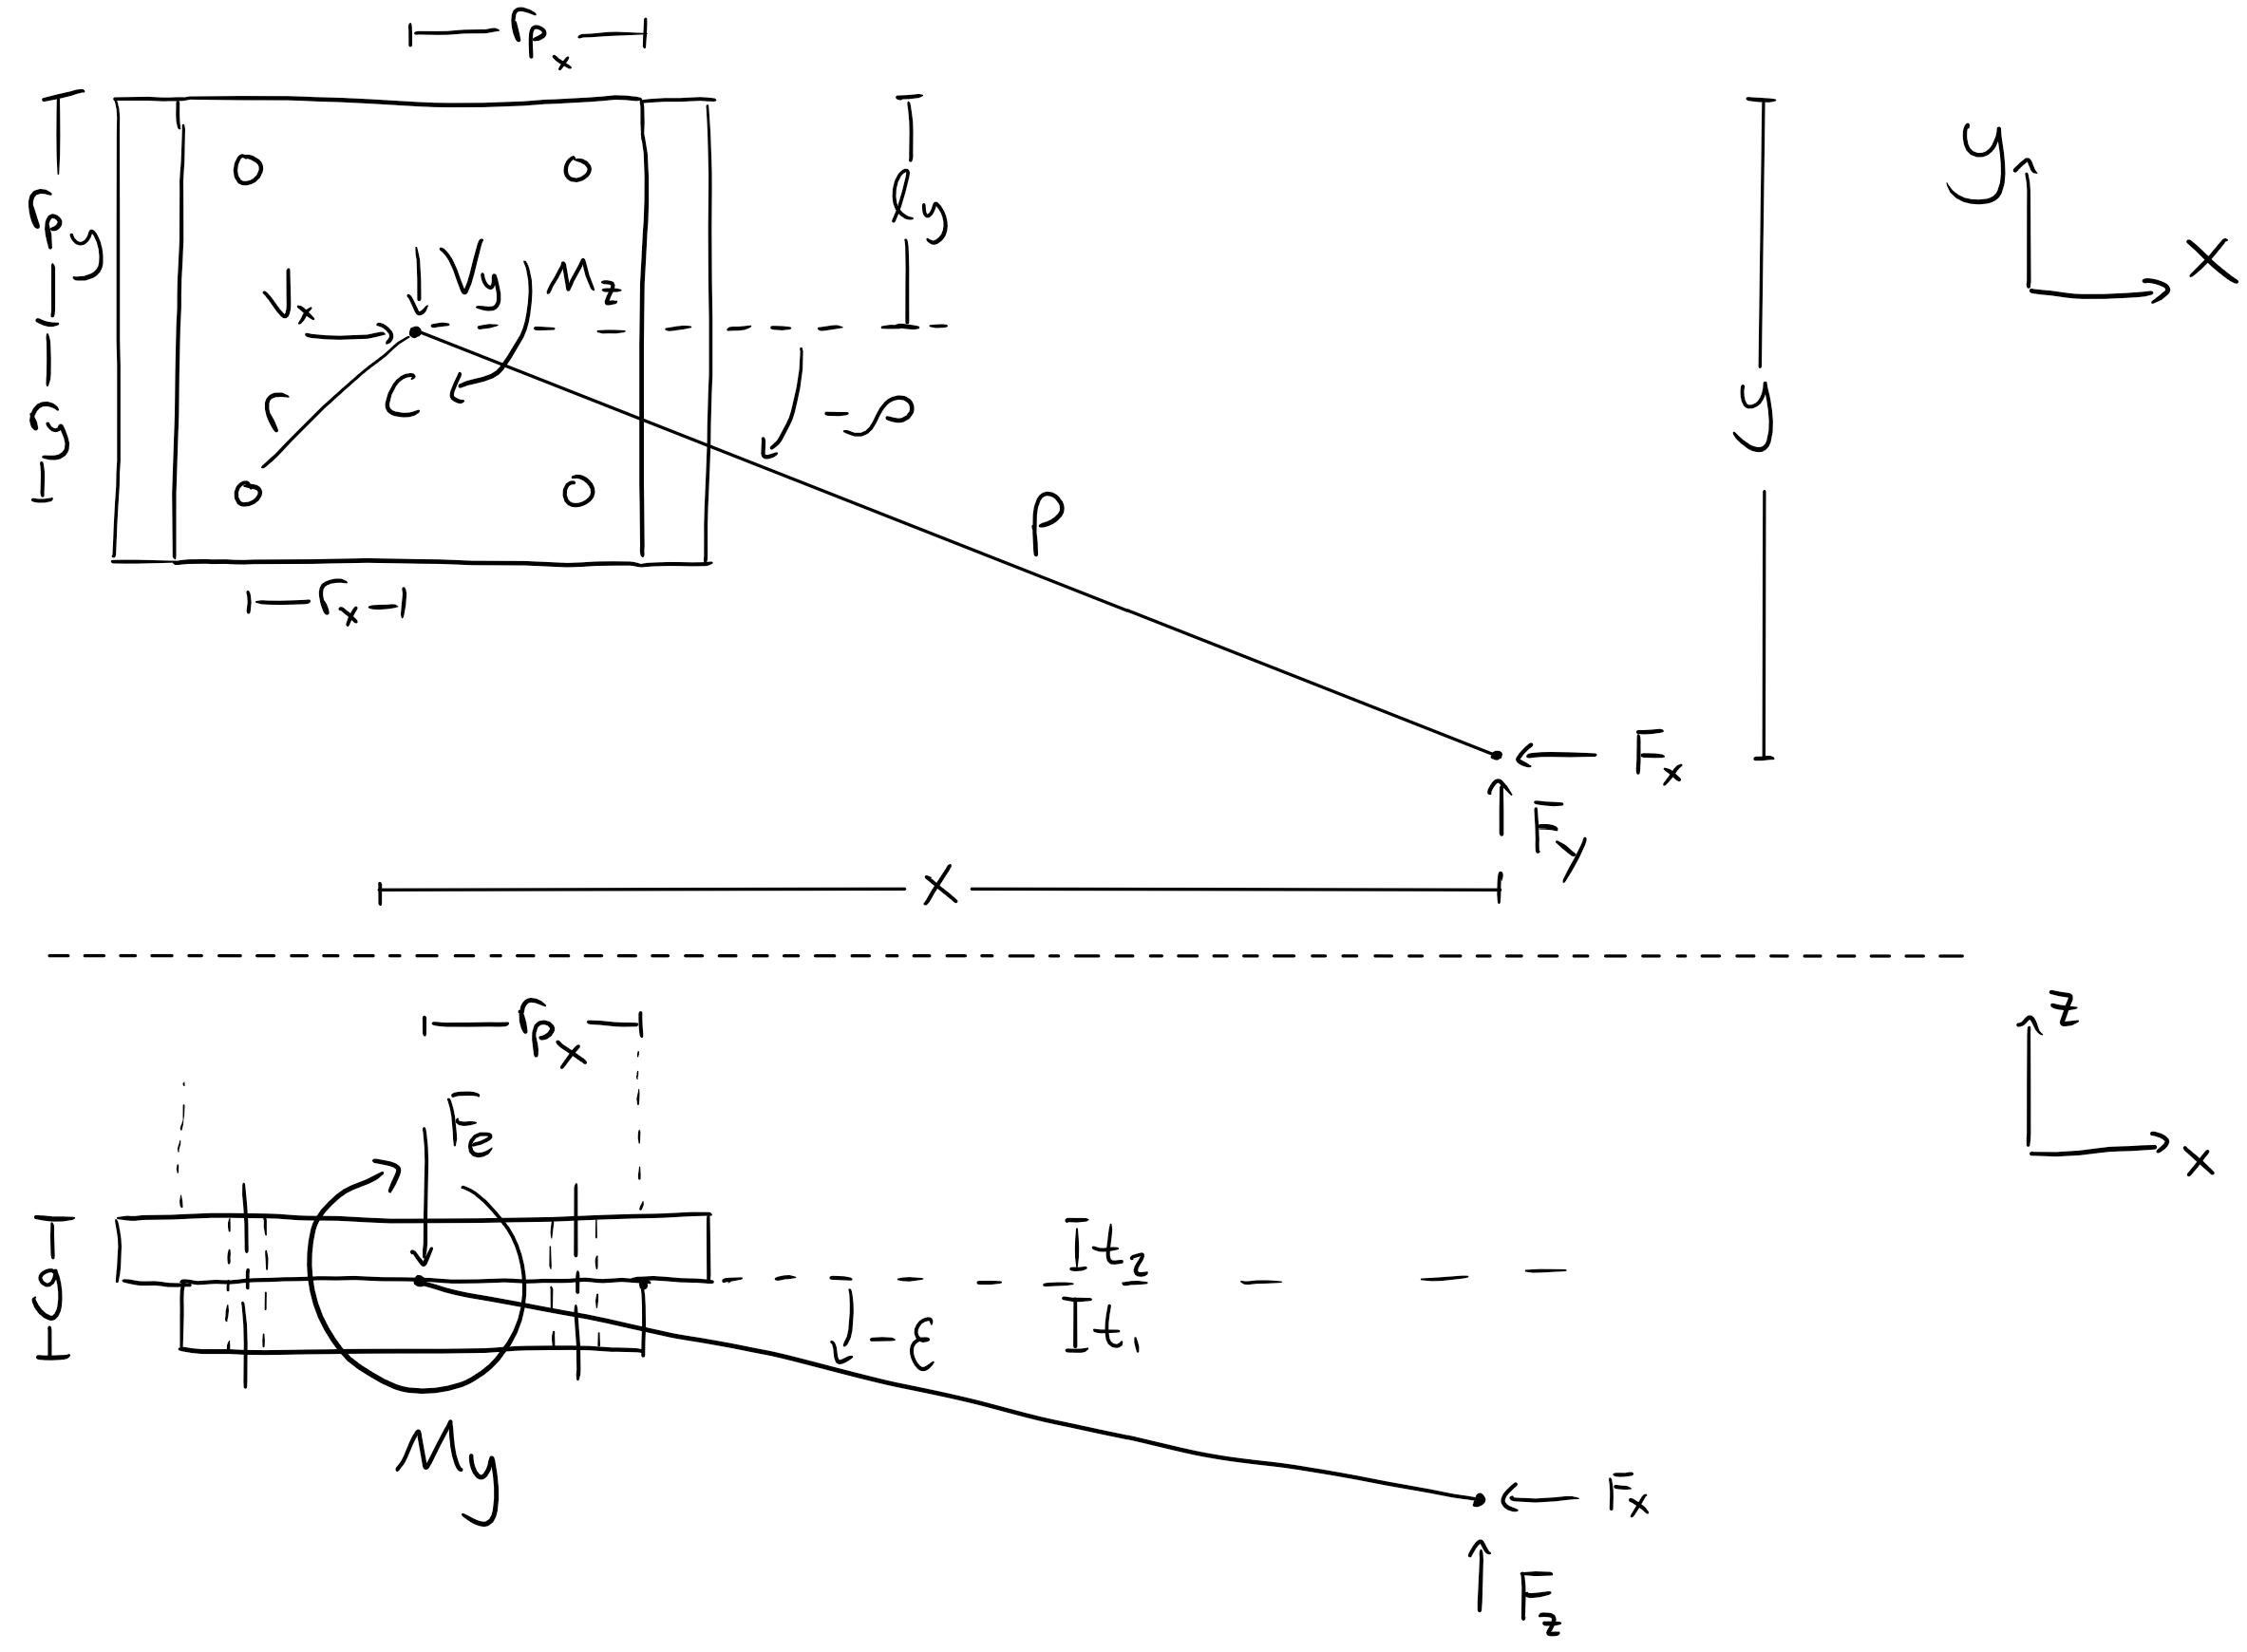
\includegraphics[width=0.85\textwidth]{4_Analysis/img/Bolts/BoltsFBDGeneral.png}
    \caption{General Free-Body Diagram for bolts}
    \label{fig:bolt_fbd_general}
\end{figure}{}

\begin{figure}
    \centering
    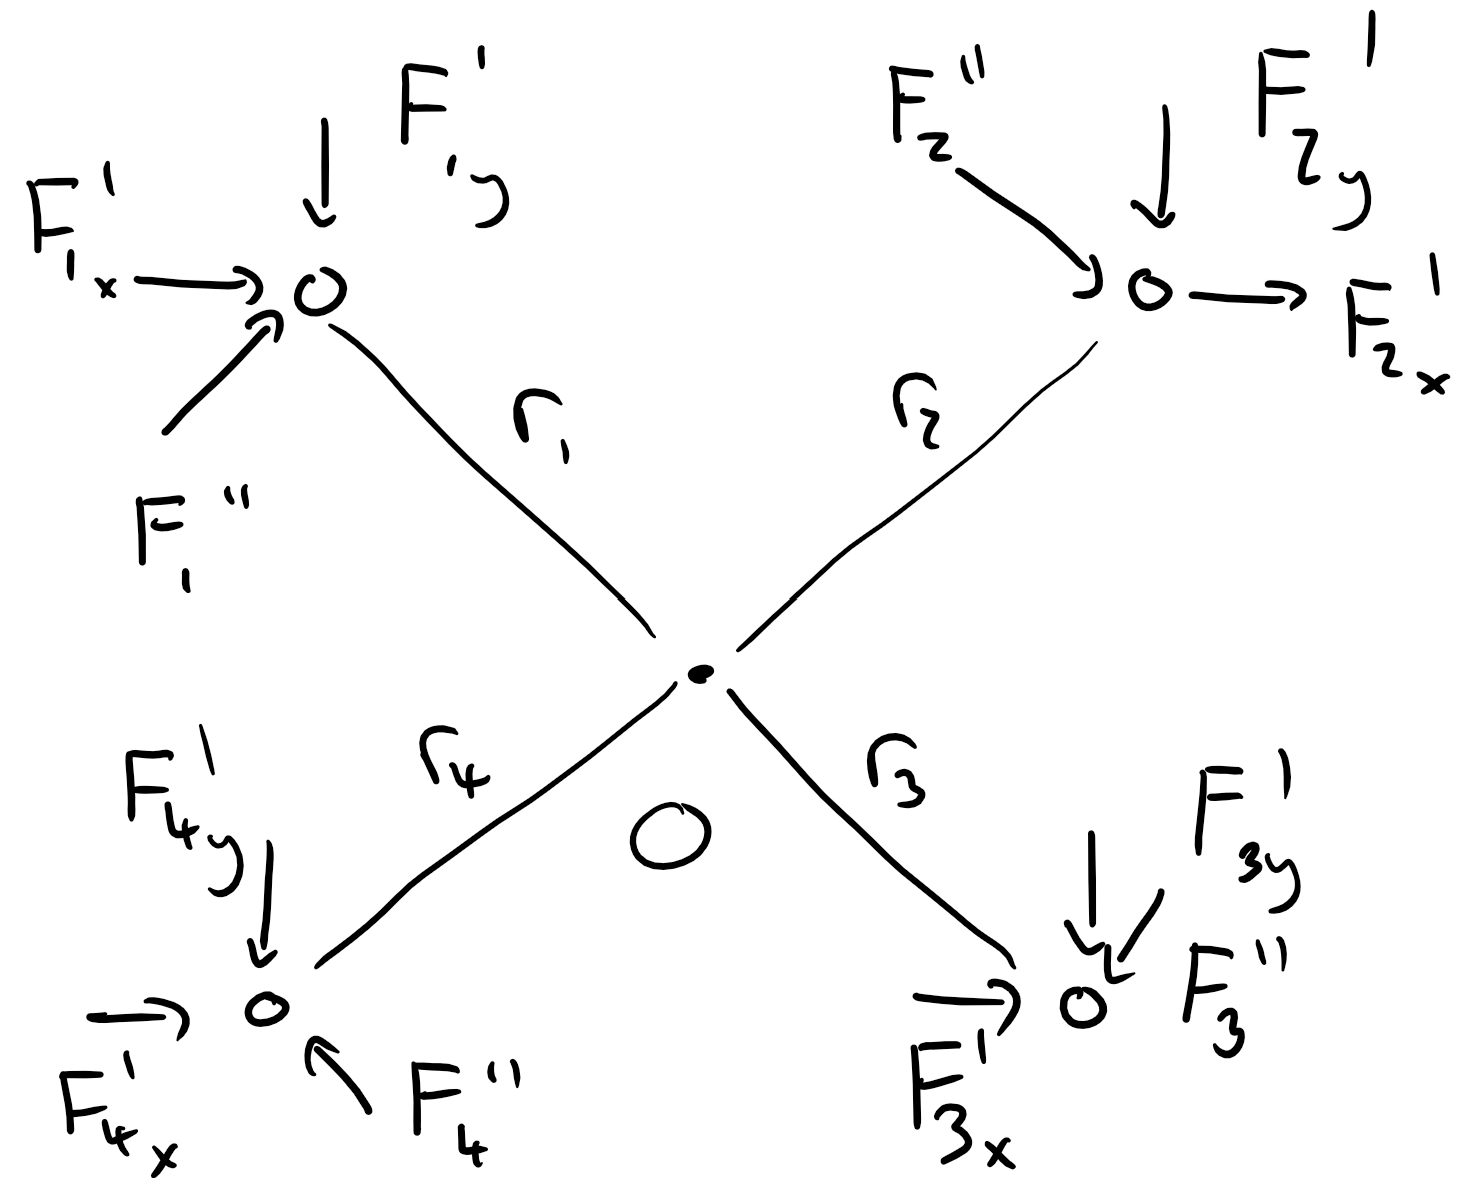
\includegraphics[width=0.5\textwidth]{4_Analysis/img/Bolts/BoltsHipShearStress.png}
    \caption{Primary and Secondary Shear Stresses in Bolts}
    \label{fig:bolt_stress}
\end{figure}

The pure shear reaction forces $V_x$ and $V_y$, tensile reaction force $F_t$ and reaction moment $M$ are.

\begin{gather}
    V_x = F_x \label{eq:bolt_reaction_shear_x}
    \\
    V_y = F_y \label{eq:bolt_reaction_shear_y}
    \\
    F_t = F_z \label{eq:bolt_reaction_shear_z}
    \\
    M_y = (F_z \cos{\epsilon} - F_x \sin{\epsilon})P \label{eq:bolt_reaction_moment_y}
    \\
    M_z = (F_y \cos{\rho} - F_x \sin{\rho}) P + T \label{eq:bolt_reaction_moment_z}
\end{gather}

Where $R$ is the distance between the applied forces and centroid of the bolts and $T$ is any pure moment applied along the member.
The centroid is located via symmetry and found to be the center of the bolts.


%------------------------------ STRESS ANALYSIS ------------------------------%
\subsubsection{Stress Analysis}

Identified failure modes include pure shear in the bolts, edge shearing of the member, crushing, tensile yielding in the bolts, and tensile yielding of the member (which will be evaluated separately in Section \ref{subsec:hipbracket}).


%------------------------------ PURE SHEAR ------------------------------%
Primary shear stresses $F'_{sh}$ and secondary shear stresses $F''_{sh}$ are shown in Figure \ref{fig:bolt_stress}.

The primary shear shear stresses are given by

\begin{equation} \label{eq:bolt_shear_force_1}
    F'_{sh}= \frac{ \sqrt{V_x^2 + V_y^2} }{n}
\end{equation}

where $n$ is the number of bolts.
Since there are 4 bolts per plate, $n=8$.
The reaction moment is given by

\begin{equation}
    M_z = F''_{sh_1} r_1 + F''_{sh_2} r_2 + \dots +  F''_{sh_n} r_n
\end{equation}

Since $r_1 = r_2 = r_3 = r_4$, the secondary shear stress is given by \cite{budynas_shigleys_2015}

\begin{equation}{} \label{eq:bolt_shear_force_2}
    F''_{sh} = \frac{M_z r}{nr^2} = \frac{M_z}{nr}
\end{equation}

Finally, the total shear force per bolt is given by

\begin{equation} \label{eq:bolt_shear_force_total}
    F_{sh} = \sqrt{{F'_{sh}}^{2} + {F''_{sh}}^{2}}
\end{equation}

And the shear stress

\begin{equation} \label{eq:bolt_shear_stress}
    \tau = \frac{F_{sh}}{A_b}
\end{equation}{}

where $A_b$ is the cross-section of the bolt along the two clamping members.
The safety factor is given by

\begin{equation} \label{eq:(SF)_bolt}
    {SF}_{sh} = \frac{S_{sy}}{\tau} = \frac{S_{sy} A_b}{F_{sh}}
\end{equation}{}

Where $S_{sy}$ is the shear yield strength, given by the Maximum-distortion-energy theory for ductile materials \cite{juvinall_fundamentals_2012}

\begin{equation} \label{eq:shear_yield_strength}
    S_{sy} = 0.58 S_y
\end{equation}{}


%------------------------------ EDGE SHEARING ------------------------------%
Edge shearing occurs when the member shears between a bolt and it's edge, usually characterized by a bolt being in too close proximity to the member's edge \cite{juvinall_fundamentals_2012}.The area for edge shearing is given by

\begin{equation}
    A_{es} = \ell_i t
\end{equation}{}

where $\ell$ is the distance from the outside of a bolt to it's edge in the direction of the applied force and $t$ is the thickness of the thinnest member.
For example, the area for edge shearing for an applied force in $x$ would give $A_{es_x} = \ell_x t$.

The shear force is given by $F_i$ from Equation \ref{eq:bolt_shear_force_total}.
The safety factor for edge shearing is given by

\begin{equation}
    (SF)_{es} = \frac{0.577 S_{y_m}}{\tau} = \frac{0.577 S_{y_m}}{\frac{F_{sh}}{A_{es_x}}} = \frac{0.577 S_{y_m} \ell_i t}{F_{sh}}
\end{equation}{}

The required distance from the edge for bolt $i$ is thus given by isolating $\ell_i$ and applying the desired safety factor.

\begin{equation} \label{eq:bolt_edge_shearing_distance}
    \ell_i = \frac{(SF)_{es} F_{sh}}{0.577 S_{y_m} t}
\end{equation}{}

Shigley recommends placing the bolts 1.5 times the diameter away from the edge; the resulting $\ell$ can be increased to match this value, or retained if above this value.\\


%------------------------------ CRUSHING ------------------------------%
The stress for bearing forces varies depending on the individual member thicknesses \cite{ahsan_mcg3131:_2018}.
For members of thickness $t_1$ and $t_2$, the bearing stresses are given by

\begin{gather}
    \sigma_1 = \frac{F_{sh}}{t_1 d}
    \\
    \sigma_2 = \frac{F_{sh}}{t_2 d}
\end{gather}{}

where $d$ is the nominal major diameter of the thread, $t_i$ is the thickness of member $i$ and $F_{sh}$ is the shear stress held by the bolt.

The safety factors for the bolt and members are given by

\begin{gather}
    (SF)_{cr_b} = \frac{S{y_b}}{\sigma_{max}}
    \\
    (SF)_{cr_1} = \frac{S{y_m}}{\sigma_1}
    \\
    (SF)_{cr_2} = \frac{S{y_m}}{\sigma_2}
\end{gather}{}

where $(SF)_{cr_b}$ is the safety factor of the bolt using the highest bearing stress $\sigma_{max}$, $(SF)_{cr_i}$ is the safety factor for member $i$, and $\sigma_i$ is the bearing stress in member $i$.
The required member thickness $t_m$ to meet the desired safety factor is then the largest of $t_m$ and $t_b$ below

\begin{gather}
    t_m = \frac{(SF)_{cr} F_{sh}}{S_{y_m} d}
    \\
    t_b = \frac{(SF)_{cr} F_{sh}}{S_{y_b} d}
\end{gather}{}


%------------------------------ TENSION ------------------------------%
The initial tension in the bolts is given by \cite{juvinall_fundamentals_2012}

\begin{equation} \label{eq:bolt_initial_tension}
    F_i = k_i A_t S_p
\end{equation}{}

where $k_i$ is a constant between 0.7 and 1.0 (chosen here to be 1.0), $A_t$ is the tensile strength area of the thread given in Table 10.2 of Juvinall and Marshek and curve-fitted with MATLAB's Curve Fitting Tool to $A_t = 0.7023d^2 - 2.669d + 9.963$, and $S_i$ is the proof strength of the material, given in Table 10.5 of Juvinall and Marshek.
The tightening torque is given by

\begin{equation}
    T = 0.2 F_i d
\end{equation}{}

where $d$ is the nominal major diameter of the thread.

With an external tensile force $F_t$, the bolt tension and clamping force are given by

\begin{gather}
    F_b = F_i + \frac{k_b}{k_b + k_m} \frac{1}{n} \left(\frac{M_y}{(r_p + r_x)} + F_t\right) \label{eq:bolts_tension_force}
    \\
    F_m = F_i - \frac{k_m}{k_b + k_m} \frac{1}{n} \left(\frac{M_y}{(r_p + r_x)} + F_t\right)
\end{gather}{}

where $F_t$ is the applied external force, $k_b$ is the spring constant of the bolt,  $k_m$ is the spring constant of the clamping members,  $\frac{M_y}{(r_p + r_x)}$ is the tension required to resist the moment $M_y$ around the pivot point $r_p$ (for the bolt the furthest from the pivot, and thus experiencing the highest stress), and $n$ is the number of bolts.
If the spring constant is unknown, it can be calculated as

\begin{gather}
    k_b = \frac{A_b E_b}{g}
    \\
    k_m = \frac{A_m E_m}{g}
\end{gather}{}

where $g$ is the effective length, shown in Figure \ref{fig:bolts_spring_constant}, and $A_b == A_t$, the nominal major area of the thread, and $E_b$ and $E_m$  are the elastic modulus of the bolt and members respectively.
In the case where multiple materials are used in the clamping members, $k_m$ can be calculated as multiple springs in series

\begin{equation}
    \frac{1}{k_m} = \frac{1}{k_{m_1}} + \dots + \frac{1}{k_{m_n}}
\end{equation}{}

where $n$ is the number of materials.
The clamping area $A_m$ can be approximated for small clearance fits with Equation \ref{eq:bolts_spring_clamping_area} \cite{juvinall_fundamentals_2012}.

\begin{equation} \label{eq:bolts_spring_clamping_area}
    A_m = d^2 + 0.68 d g + 0.065 g^2
\end{equation}{}

\begin{figure}
    \centering
    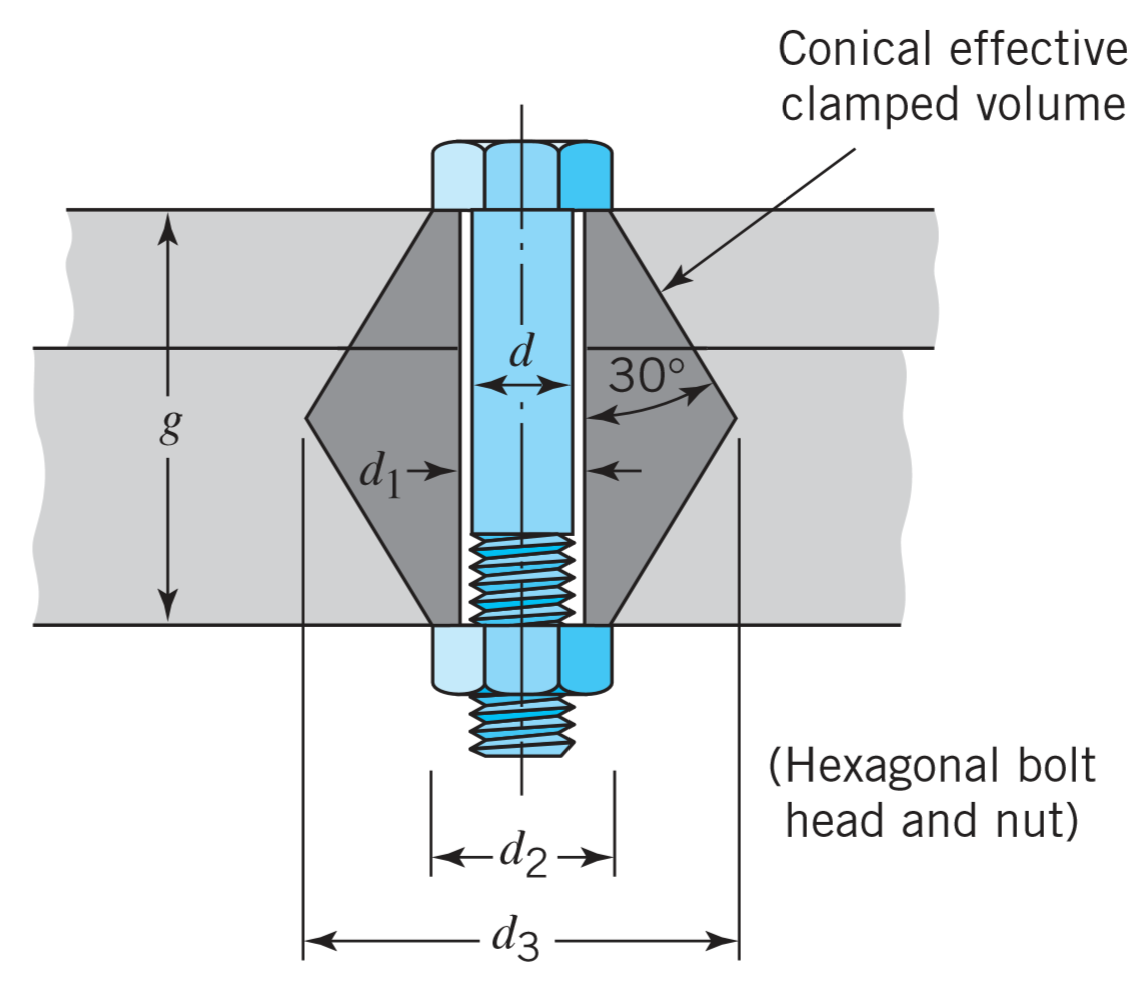
\includegraphics[width=0.5\textwidth]{4_Analysis/img/Bolts/BoltTensionDiagram.png}
    \caption{Determining spring constant of bolt and clamping member \cite{juvinall_fundamentals_2012}}
    \label{fig:bolts_spring_constant}
\end{figure}{}

Finally, the safety factor is given by

\begin{equation}
    {SF}_t = \frac{S_{y_b}}{\sigma}
\end{equation}{}

It was found that the safety factor sits around 2.2 regardless of the external load; this is likely because the initial tension of the bolt is significantly larger than the external forces, and thus they have little impact on the safety factor.
A factor as low as two is allowed for tension.
For cases where the bolts do not all have the same distance $r_p+r_x$, then only the number of bolts at distance $r_p+r_x$ should be considered.


%------------------------------ FATIGUE ------------------------------%
\begin{comment}{}
    Tensile fatigue is another major failure source for bolts \cite{budynas_shigleys_2015}.
    The fatigue stress safety factor for 4.8 metric bolts is $k_f = 2.8$.
    The stiffness constant $C$ of the bolt is given by
    
    \begin{equation}
        C = \frac{k_b}{k_b + k_m}
    \end{equation}{}
    
    The alternating stress and midrange stress experienced by a bolt are respectively
    
    \begin{gather}
        \sigma_a = \frac{C(F_{t_{max}} - F_{t_{min}})}{2A_t}
        \\
        \sigma_m = \frac{C(F_{t_{max}} + F_{t_{min}})}{2A_t} + \frac{F_i}{A_t}
    \end{gather}{}
    
    where $F_{t_max}$ is the maximum external tensile force experienced by the bolt, $F_{t_max}$ is the minimum external tensile force applied to the bolt, $A_t$ is the tensile strength area of the thread given in Table 10.2 of Juvinall and Marshek, and $F_i$ is the initial bolt tension as per Equation \ref{eq:bolt_initial_tension}.
    Using the modified Goodman criteria, the safety factor for fatigue is given by
    
    \begin{equation}
        (SF)_{f} = \frac{S_e (S_{ut} - \sigma_i)}{S_{ut} \sigma_a + S_e (\sigma_m - \sigma_i)}
    \end{equation}{}
    
    where $S_e$ is the fully corrected fatigue strength of bolts from Table 8-17 of Shigley, $S_{ut}$ is the ultimate tensile strength of the bolt and $\sigma_i$ is the initial stress by preloading (determined using $F_i$ from Equation \ref{eq:bolt_initial_tension}) and $A_t$, the tensile strength area of the bolt.
\end{comment}


%------------------------------ EXAMPLE ------------------------------%
\subsubsection{Example}

\begin{figure}
    \centering
    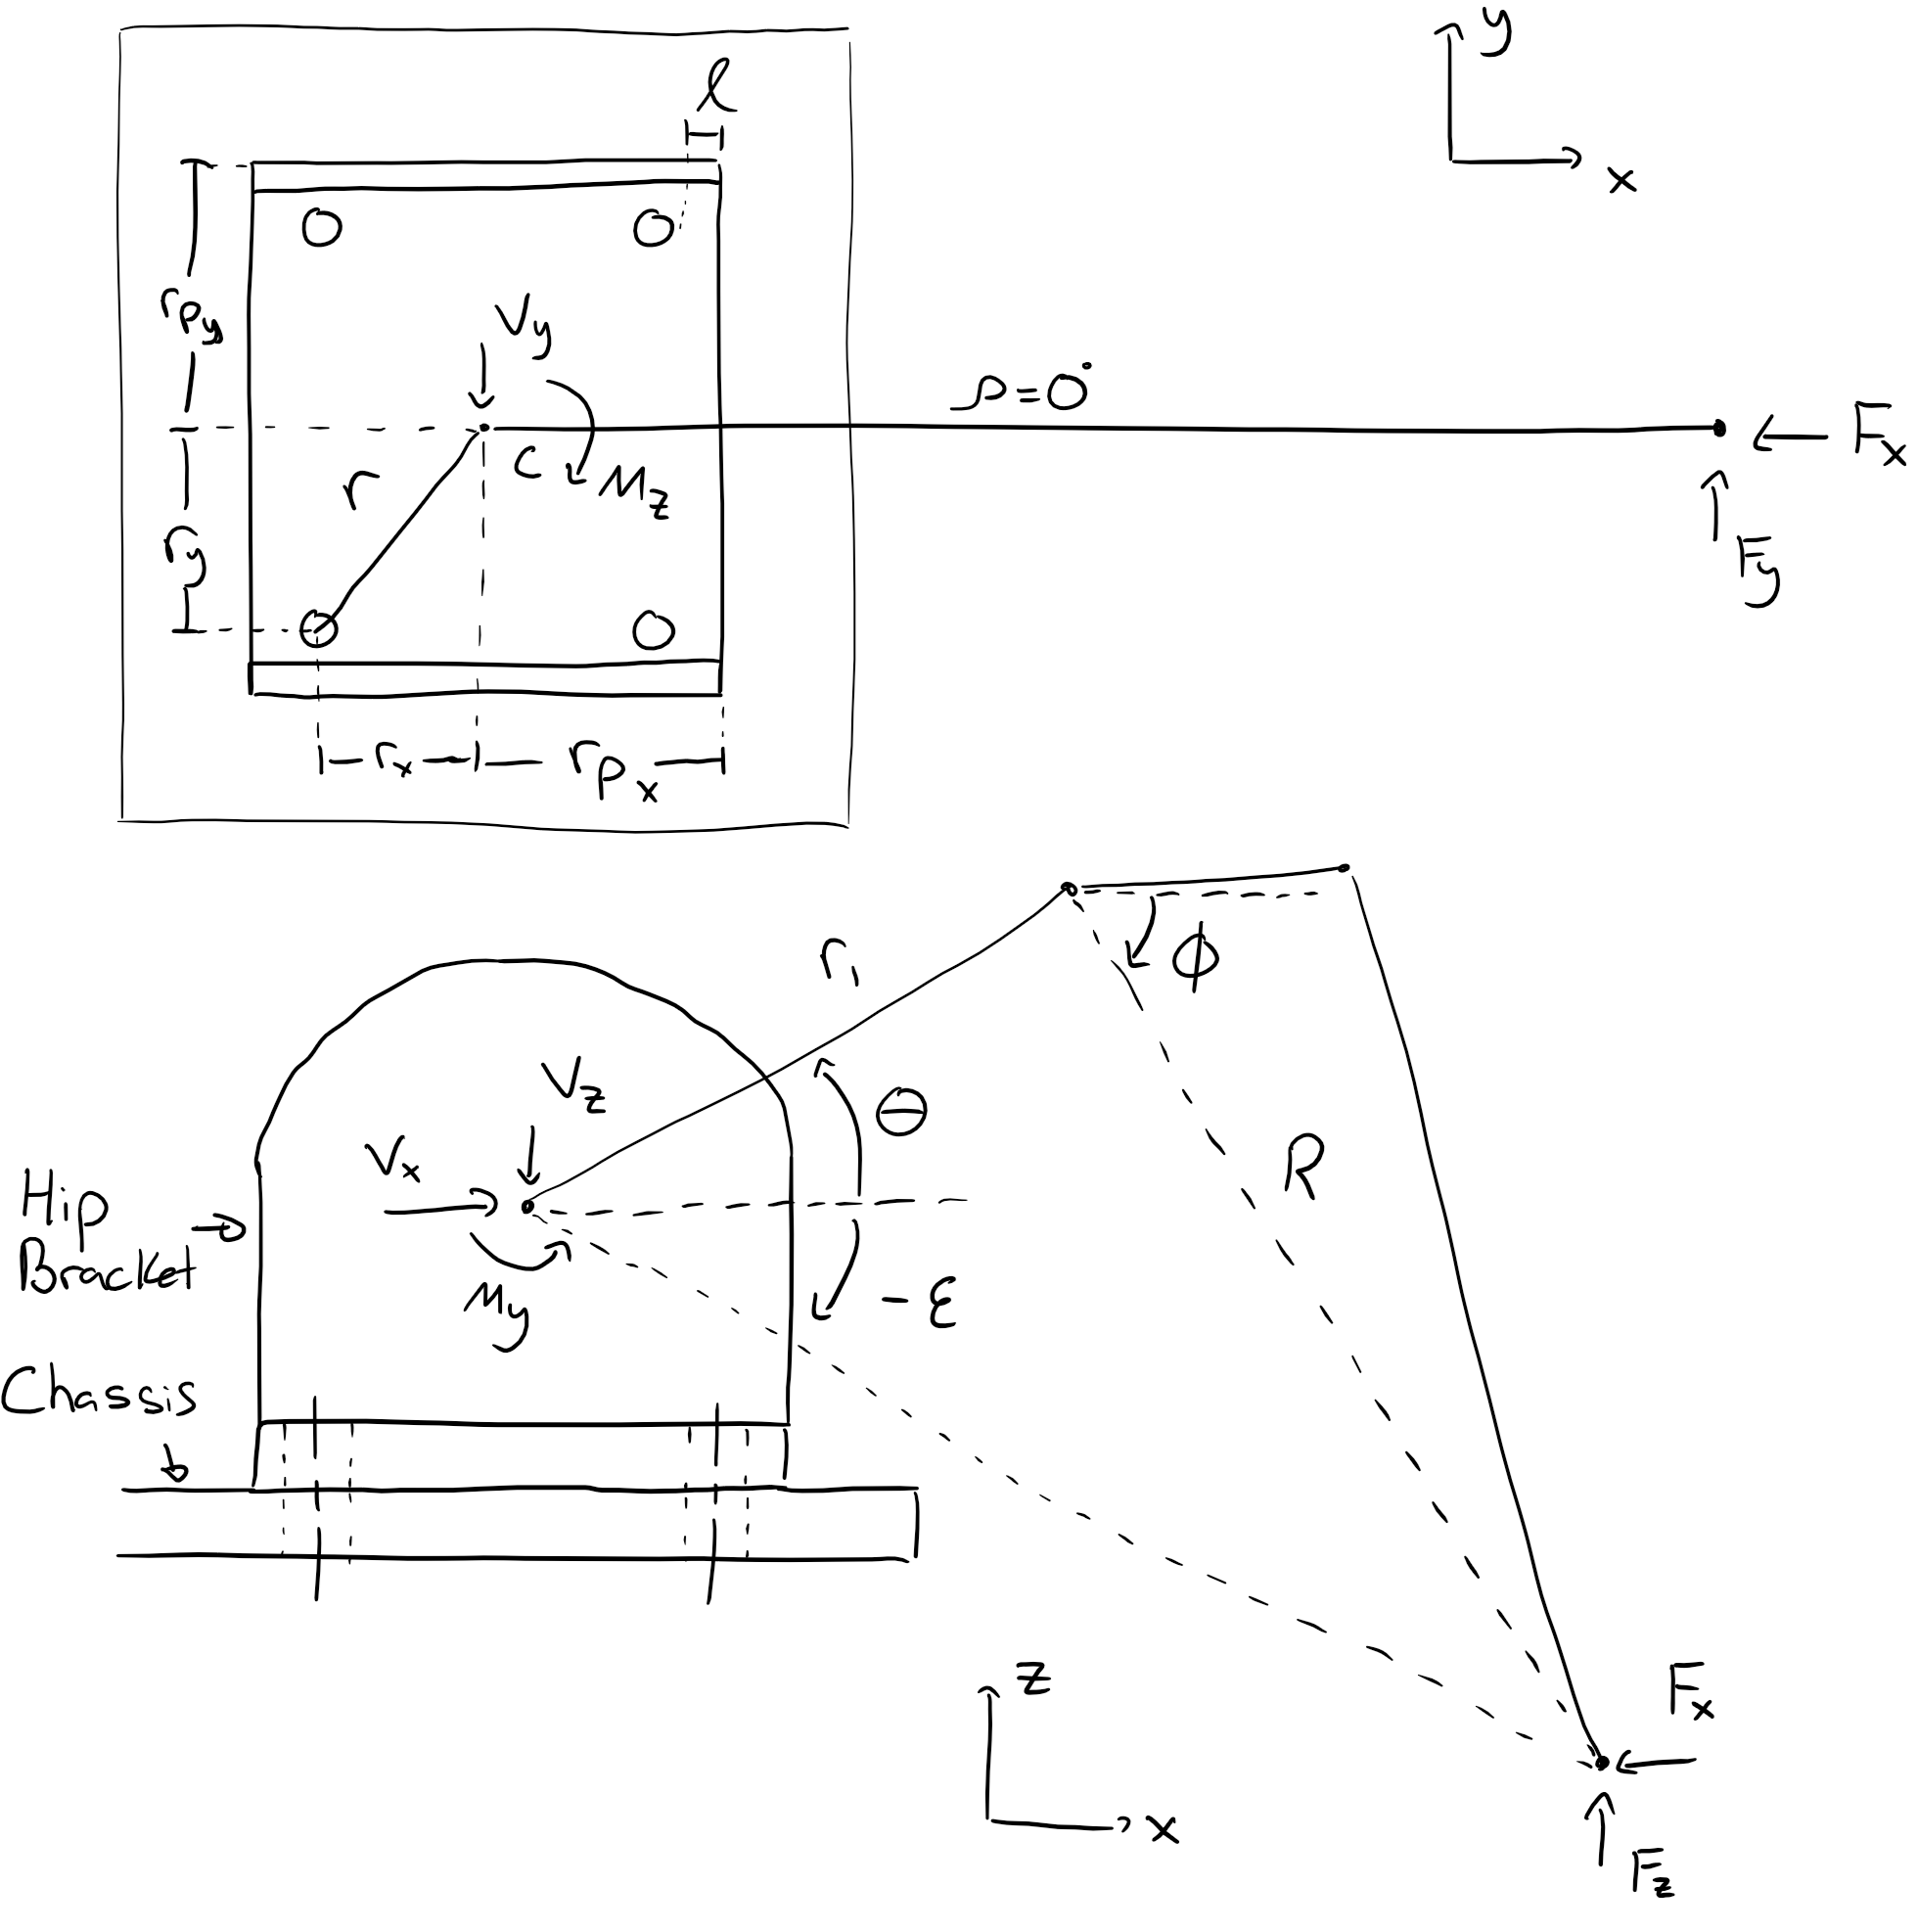
\includegraphics[width=0.7\textwidth]{4_Analysis/img/Bolts/BoltsHipFBD.png}
    \caption{Force-Body Diagram of hip bolts}
    \label{fig:bolt_fbd_hip}
\end{figure}

The following example illustrates the stress analysis for the fasteners holding the hip plates and motor to the chassis, illustrated in Figure \ref{fig:bolt_fbd_hip}.
The clamping members are assumed to be made of Aluminium 6061, with a yield strength of $276MPa$ \cite{matweb_aluminum_nodate}, and a thickness of an eighth inch for each member ($3.175mm$), giving $g = t_1+t_2 = 6.35mm$.
The bolts are made of medium carbon steel (class 9.8), with an elastic modulus of approximately $200MPa$ \cite{azom_aisi_2012}.
The most extreme case for loading on a bolt is the maximum robot size (5kg of litter) with the leg fully extended, when $\theta = 17.18^{\circ}$, $\phi=-51.89^{\circ}$ (from horizontal), $r_1 = 100mm$, $R = 280.17mm$.
$r$ is assumed to be $70.71mm$ and $r_p$ is assumed to be $70mm$.
The initial bolt diameter is estimated to by $5mm$ (M5).
The mechanical properties of class 9.8 steel is found in Table \ref{tab:bolts_material}.
In this case, we can compute the moment arm $P$ and angle of application $\rho$ as

\begin{gather}
    x = r_1 \cos{\theta} + R\cos{\phi} = 268.44 mm
    \\
    y =  0 mm
    \\
    z = r_1 \sin{\theta} + R\sin{\phi} = -190.9012 mm
    \\
    \rho = 0^{\circ}
    \\
    \epsilon = \arctan \big( \frac{z}{x} \big) = -35.41^{\circ}
\end{gather}{}

\begin{equation}
    \begin{split}
        P   &= \sqrt{ r_1^2 + R^2 - 2 r_1 R \cos(\phi-\theta-\pi) } \\
            &= \sqrt{ (100mm)^2 + (280.17mm)^2 - 2\cdot 100^{\circ} \cdot 280.17 \cos(-51.89^{\circ} - 17.18^{\circ} - \pi)} \\
            &= 329.40 mm
    \end{split}
\end{equation}

with maximum foot forces given by

\begin{gather}
    F_x = 100N
    \\
    F_y = 100N
    \\
    F_z = 160N
\end{gather}{}

With $F_z$ being the normal force when on flat ground (maximum), $F_x$ being the maximum friction force in the $x$ direction and $F_y$ being the maximum friction force in the $y$ direction, while on a $20^{\circ}$ incline.
Both friction forces will never occur simultaneously, as $100N$ is the total friction amplitude and would thus be split between them, however this gives a conservative estimate.
Equally, the maximum normal and friction forces will never occur simultaneously, however for the sake of being conservative both are considered here simultaneously.

The reaction forces and moment are thus

\begin{gather}
    V_x = 100N
    \\
    V_y = 100N
    \\
    V_z =  160N
    \\
    M_y = ((100N)\cos(0^{\circ}) - (100N)\sin(0^{\circ}))(280.17mm) =  62041Nmm
    \\
    M_z = ((160N)\cos(-35.41^{\circ}) - (100N)\sin(-35.41^{\circ}))(280.17mm) = 32940Nmm
\end{gather}{}

As there are 4 bolts, $n=4$.

Primary, secondary and total shear stress per bolt are given as

\begin{gather}
    F'_sh = \frac{\sqrt{(100N)^2 + (100N)^2}}{4{bolts}} = 35.35N
    \\
    F''_sh = \frac{32940Nmm}{(4\text{bolts}(70.71mm)} = 116.46N
    \\
    F_sh = \sqrt{(35.35N)^2 + (116.46N)^2} = 121.70N
\end{gather}{}

The safety factor in shear is thus given by

\begin{equation}
    (SF)_{sh} = \frac{0.58\pi  (340MPa)(5mm)^2}{4 (121.70N)} = 67.36
\end{equation}{}

The given bolt diameter and radius from bolt to centroid are more than sufficient for shear stress.

The required member thicknesses are then calculated to resist bearing/crushing forces

\begin{equation}
    t_{m} = \frac{2.5(121.70N)}{(276MPa)(5mm)} = 0.2205mm
\end{equation}{}

The members can be very thin and still resist bearing forces.
Next, the required distance from the extremity of the bolts to the edges is calculated to resist edge shearing.

\begin{equation}
    \ell = \frac{2.5(121.70N)}{0.577(276MPa)(0.2205mm)} = 8.66mm
\end{equation}{}

It is worth noting that increasing the member thickness decreases the required distance from the edge (for example, doubling the member thickness would half $\ell$).
We can therefore increase the member thickness to the initial 3.175mm, giving $\ell=0.6018$.

The bolt is then evaluated for tensile loads.
The initial bolt tension and tightening torque are given by

\begin{gather}
    F_i = 0.7(14.175mm^2)(650MPa) = 6449.9N
    \\
    T = 0.2 (6449.9N) (5mm) = 6449.9N
\end{gather}{}

The spring constants of the bolt and member are respectively

\begin{gather}
    A_b = \frac{\pi(5mm)^2}{4} = 19.635mm^2
    \\
    k_b = \frac{(19.635mm^2)(200MPa)}{2(3.175mm)} = 618.42\frac{N}{mm}
    \\
    A_m \approx (5mm)^2 + 0.68(5mm)(6.35mm) + 0.065(6.35mm)^2 = 49.21mm^2
    \\
    k_m = \frac{(78.663mm^2)(276MPa)}{2(3.175mm)} = 2138.93\frac{N}{mm}
\end{gather}{}

Finally, the tensile forces in the bolt and members are given by

\begin{gather}
    F_b = 6449.9N + \frac{618.42\frac{N}{mm}}{618.42\frac{N}{mm} + 2138.93\frac{N}{mm}} \frac{1}{4\text{bolts}} \left( 160N + \frac{62041Nmm}{(70mm) + (50mm)} \right) = 6487.81N
    \\
    F_m = 6449.9N - \frac{618.42\frac{N}{mm}}{618.42\frac{N}{mm} + 2138.93\frac{N}{mm}} \frac{1}{4\text{bolts}} \left( 160N + \frac{62041Nmm}{(70mm) + (50mm)} \right) = 6318.55N
\end{gather}{}

The applied force has little impact on the force felt by the member or bolt; the initial tension is still much larger.
The safety factor in tension for the bolt is

\begin{gather}
    \sigma_b = \frac{4(6487.81N)}{\pi(5mm)^2} = 330.42MPa
    \\
    SF = \frac{720MPa}{329.616MPa} = 2.17
\end{gather}{}

This is below the desired 2.5 safety factor, however as noted in the stress analysis, the initial tension in the bolts is responsible for most of the stress, and thus applied loads barely influence the safety factor; the design goal for tension is a safety factor of 2, not 2.5.


%------------------------------ CRITICAL REVIEW ------------------------------%
\subsubsection{Critical Review}

Shear failure is very unlikely; the safety factor was much higher for pure shear than pure tension.
Both the shear and tensile safety factors are inversely proportionate to the distance between the bolts and their centroid, $r$; in order to minimize space and maintain an acceptable safety factor, the distance $r$ and the bolt diameter $d$ must be determined through iteration.

The distance from bolt to edge $\ell$ and member thickness $t_m$ are inversely proportionate.
Since the minimum required member thickness is small, and since the chassis dimensions depends more on the $x$ and $y$ dimensions of internal components ($z$ is mostly dependant on the size of the knee harmonic drive and motor, and clearance needed for them to rotate $45^{\circ}$) it can be increased to a more reasonable value, saving space in the $x-y$ plane.

The safety factor in tension is less important for this assembly, it seems.
Even with the normal force $F_z$ increased by a factor of 100, the safety factor in tension is above $1.5$; the majority of the loading in the bolts is still from the initial tightening, and thus the required safety factor has been lowered to $2$
The safety factor in shear is more volatile, however, and given large loads or very small bolt diameters and $r$, it can pass below $2.5$.
The methodology presented above is somewhat limited, in that it assumes that the bolts follow a square configuration.

Some geometry was ignored.
For example, when calculating the forces in tension, the load was evenly divided between the bolts. This is not correct, as the bolts furthest from the pivot point would take more force than those closer.
Since the safety factor in tension does not vary until increasing the applied load by a couple orders of magnitude, this simplification is acceptable.

In terms of the example, the height of $150mm$ between the motor in the bolts was forgotten.
This would have reduced the tensile moment, however, and so does not negatively impact the safety factor of the analysis.


%------------------------------ PARAMETRIZATION ------------------------------%
\subsubsection{Parameterization}

The values of $r$, $d$, $t_m$ and $\ell$ are determined by first generating a range of values for all four, then creating 4D matrices with the following 2D principle extended to 4D:

\begin{gather}
    \text{Matrix}_r = 
    \begin{bmatrix}{}
        r_1 & r_1 & \dots & r_1 \\
        r_2 & r_2 & \dots & r_2 \\
        \dots  &  &       & \dots \\
        r_n & r_n & \dots & r_n
    \end{bmatrix}
    \\
    \text{Matrix}_d = 
    \begin{bmatrix}{}
        d_1 & d_2 & \dots & d_n \\
        d_1 & d_2 & \dots & d_n \\
        \dots & & & \dots \\
        d_1 & d_2 & \dots & d_n \\
    \end{bmatrix}
\end{gather}{}

The stress analysis functions are then applied to each combination of $r$, $d$, $t_m$ and $\ell$ and the one that minimizes some measure of space occupied (such as minimizing the area occupied by the bolts) while maintaining the desired safety factors of $2$ for tension and $2.5$ for everything else will be selected.